% Source: graduate-coursework/Research/Intro_to_Agents/handouts/Part5_TwoLayer_Agents.tex

\documentclass[border=4pt]{standalone}
\usepackage[T1]{fontenc}
\usepackage{graphicx}
\usepackage{lmodern}
\usepackage{tikz}
\usepackage{xcolor}
\usetikzlibrary{shapes.geometric, arrows.meta, positioning, fit, calc, backgrounds}

\definecolor{UofSCGarnet}{HTML}{73000a}
\definecolor{UofSCBlack}{HTML}{000000}
\definecolor{UofSCWhite}{HTML}{ffffff}
\definecolor{UofSCRose}{HTML}{CC2E40}
\definecolor{UofSCAtlantic}{HTML}{466A9F}
\definecolor{UofSCCongaree}{HTML}{1F414D}
\definecolor{UofSCHorseshoe}{HTML}{65780B}
\definecolor{UofSCGrass}{HTML}{CED318}
\definecolor{UofSCHoneycomb}{HTML}{A49137}
\definecolor{UofSC90Black}{HTML}{363636}
\definecolor{UofSC70Black}{HTML}{5C5C5C}
\definecolor{UofSC50Black}{HTML}{A2A2A2}
\definecolor{UofSCWarmGrey}{HTML}{676156}
\definecolor{UofSCSandstorm}{HTML}{FFF2E3}
\definecolor{UofSCDarkGarnet}{HTML}{570008}
\definecolor{UofSCAzalea}{HTML}{844247}

\tikzset{
    % Box styles - all sharp corners
    orchestrator/.style={
        rectangle,
        draw=UofSCGarnet,
        fill=UofSCGarnet!10,
        line width=1.5pt,
        minimum width=4cm,
        minimum height=1.2cm,
        align=center,
        font=\bfseries
    },
    worker/.style={
        rectangle,
        draw=UofSCAtlantic,
        fill=UofSCAtlantic!10,
        line width=1pt,
        minimum width=2cm,
        minimum height=0.9cm,
        align=center
    },
    task/.style={
        rectangle,
        draw=UofSCCongaree,
        fill=UofSCCongaree!10,
        line width=1pt,
        minimum width=1.8cm,
        minimum height=0.8cm,
        align=center
    },
    process/.style={
        rectangle,
        draw=UofSCBlack,
        fill=UofSCWhite,
        line width=1pt,
        minimum width=3cm,
        minimum height=0.8cm,
        align=center
    },
    result/.style={
        rectangle,
        draw=UofSCHorseshoe,
        fill=UofSCHorseshoe!10,
        line width=1pt,
        minimum width=2.5cm,
        minimum height=0.8cm,
        align=center
    },
    decision/.style={
        diamond,
        draw=UofSCGarnet,
        fill=UofSCGarnet!10,
        line width=1pt,
        minimum width=2cm,
        minimum height=1cm,
        align=center,
        aspect=2
    },
    % Arrow styles - straight lines only
    arrow/.style={
        ->,
        >=Stealth,
        line width=1pt,
        draw=UofSCBlack
    },
    thickarrow/.style={
        ->,
        >=Stealth,
        line width=1.5pt,
        draw=UofSCGarnet
    },
    dashedarrow/.style={
        ->,
        >=Stealth,
        line width=1pt,
        draw=UofSC70Black,
        dashed
    }
}

\begin{document}
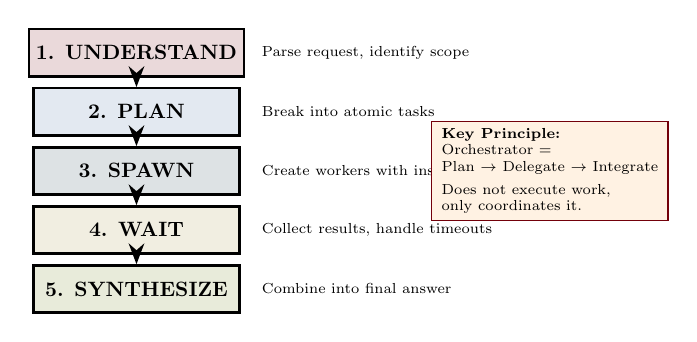
\begin{tikzpicture}[scale=0.75, transform shape]
    % Workflow steps
    \node[process, fill=UofSCGarnet!15, minimum width=3.5cm] (u) at (0,3.5) {\textbf{1. UNDERSTAND}};
    \node[font=\scriptsize, anchor=west] at (2,3.5) {Parse request, identify scope};

    \node[process, fill=UofSCAtlantic!15, minimum width=3.5cm] (p) at (0,2.5) {\textbf{2. PLAN}};
    \node[font=\scriptsize, anchor=west] at (2,2.5) {Break into atomic tasks};

    \node[process, fill=UofSCCongaree!15, minimum width=3.5cm] (s) at (0,1.5) {\textbf{3. SPAWN}};
    \node[font=\scriptsize, anchor=west] at (2,1.5) {Create workers with instructions};

    \node[process, fill=UofSCHoneycomb!15, minimum width=3.5cm] (w) at (0,0.5) {\textbf{4. WAIT}};
    \node[font=\scriptsize, anchor=west] at (2,0.5) {Collect results, handle timeouts};

    \node[process, fill=UofSCHorseshoe!15, minimum width=3.5cm] (sy) at (0,-0.5) {\textbf{5. SYNTHESIZE}};
    \node[font=\scriptsize, anchor=west] at (2,-0.5) {Combine into final answer};

    % Arrows
    \draw[arrow] (u) -- (p);
    \draw[arrow] (p) -- (s);
    \draw[arrow] (s) -- (w);
    \draw[arrow] (w) -- (sy);

    % Side annotations
    \node[draw=UofSCGarnet, fill=UofSCSandstorm, align=left, font=\scriptsize, minimum width=4cm] at (7,1.5) {
        \textbf{Key Principle:}\\
        Orchestrator = \\
        Plan $\rightarrow$ Delegate $\rightarrow$ Integrate\\[3pt]
        Does not execute work,\\
        only coordinates it.
    };
\end{tikzpicture}
\end{document}
